\documentclass[11pt, reqno]{amsart}
\usepackage{amsfonts, amssymb, amscd}
%\usepackage{amsrefs}
\usepackage{graphicx}
\usepackage{hyperref}
\usepackage{slashed}
\usepackage{fullpage}
% Prevent table repositioning.
\usepackage{float}
% For textcolor.
\usepackage{xcolor}
% For blackboard bold `1`.
\usepackage{bbold}

\usepackage{booktabs}
\usepackage{tabularx}
\usepackage{longtable, array}

\usepackage{algorithm}
\usepackage{algpseudocode}

\usepackage{makecell}

%\usepackage{titlesec}

%\titleformat*{\section}{\LARGE\bfseries}
%\titleformat*{\subsection}{\Large\bfseries}
%\titleformat*{\subsubsection}{\large\bfseries}
%\titleformat*{\paragraph}{\large\bfseries}
%\titleformat*{\subparagraph}{\large\bfseries}

% If you need math, theorems, etc.
\usepackage{amsmath, amssymb, amsthm}
\usepackage{tikz}
\usetikzlibrary{
  positioning,
  calc,
  arrows.meta,
  decorations.pathreplacing
}

\usepackage[useregional]{datetime2}
\DTMlangsetup[en-US]{zone=eastern,mapzone}

% --- Theorem environments (acmart loads amsthm; this is safe) ---
\theoremstyle{plain}
\newtheorem{theorem}{Theorem}[section]
\newtheorem{lemma}[theorem]{Lemma}
\newtheorem{proposition}[theorem]{Proposition}
\newtheorem{corollary}[theorem]{Corollary}

\theoremstyle{definition}
\newtheorem{definition}[theorem]{Definition}

\theoremstyle{remark}
\newtheorem{remark}[theorem]{Remark}

\newtheorem{assumption}{Assumption}[section]

\input{./helpers_root/dev_scripts_helpers/documentation/latex_abbrevs.sty}

% Python style for highlighting
\usepackage{listings}

\newcommand{\pythonstyle}{\lstset{ language=Python, basicstyle=\ttm, morekeywords={self}, % Add keywords here
keywordstyle=\ttb
\color{deepblue}
, emph={MyClass,__init__}, % Custom highlighting
emphstyle=\ttb
\color{deepred}
, % Custom highlighting style
stringstyle=
\color{deepgreen}
, frame=tb, % Any extra options here
showstringspaces=false }}

% Python environment.
\lstnewenvironment{python}[1][]{ \pythonstyle \lstset{#1} }{}

% Python for external files.
\newcommand{\pythonexternal}[2][]{{ \pythonstyle \lstinputlisting[#1]{#2}}}

% Python for inline.
\newcommand{\pythoninline}[1]{{\pythonstyle\lstinline!#1!}}

\usepackage{listings}
\usepackage{xcolor}

\definecolor{codegreen}{rgb}{0,0.6,0}
\definecolor{codegray}{rgb}{0.5,0.5,0.5}
\definecolor{codepurple}{rgb}{0.58,0,0.82}
\definecolor{backcolour}{rgb}{0.95,0.95,0.92}

\lstdefinestyle{mystyle}{ backgroundcolor=
\color{backcolour}
, commentstyle=
\color{codegreen}
, keywordstyle=
\color{magenta}
, numberstyle=\tiny
\color{codegray}
, stringstyle=
\color{codepurple}
, basicstyle=\ttfamily\footnotesize, breakatwhitespace=false, breaklines=true, captionpos=b,
keepspaces=true, numbers=left, numbersep=5pt, showspaces=false, showstringspaces=false,
showtabs=false, tabsize=2 }

\lstset{style=mystyle}

% end python

%

\providecommand{\tightlist}{%
\setlength{\itemsep}{0pt}
\setlength{\parskip}{0pt}}

% Use this if using `\contrib[]{...}`.
%\makeatletter\let\@wraptoccontribs\wraptoccontribs\makeatother
% https://tex.stackexchange.com/questions/418547/equal-contribution-using-thanks-with-llncs-class#418563
\makeatletter
\newcommand{\printfnsymbol}[1]{%
\textsuperscript{\@fnsymbol{#1}}%
}
\makeatother


\begin{document}
  \title{A Theoretical Framework for Quantifying Skill and Luck in Agent
  Outcomes}

  \author{Giacinto Paolo Saggese$^{*}$}
  \thanks{$^{*}$ Causify.AI, The University of Maryland, College Park, MD 20742, USA, gsaggese@umd.edu}

  \date{\today}

  \maketitle

  \begin{abstract}
    The inability to rigorously separate skill from luck in human outcomes represents
    perhaps the most consequential unsolved problem in social science, underpinning
    every question of justice, merit, responsibility, and institutional design.
    Despite millennia of philosophical inquiry and centuries of statistical analysis,
    we have lacked the mathematical foundation to quantify what portion of observed
    inequality reflects genuine differences in ability versus the capricious distribution
    of fortune. This paper provides that foundation.

    We develop the first complete mathematical framework for decomposing agent outcomes
    into skill and luck components by integrating probability theory, decision theory,
    and causal inference. Our formalization defines luck as value-weighted surprise
    of outcomes not explained by controllable factors, enabling principled measurement
    of both individual events and population-level distributions. This framework
    fundamentally transforms our ability to address questions that have remained
    intractable: How much of economic inequality is attributable to circumstances
    versus choices? What degree of outcome variation lies beyond individual control?
    How should institutions account for luck when evaluating performance and allocating
    resources?

    The implications are profound and far-reaching. This framework provides the missing
    analytical foundation for understanding social stratification, meritocracy, and
    distributive justice. It enables evidence-based policy design by quantifying
    the extent to which outcomes reflect factors beyond individual agency. It offers
    a rigorous basis for moral philosophy's treatment of responsibility and desert.
    And it supplies the tools necessary for evaluating whether our institutions
    reward skill or merely reinforce the accidents of birth and circumstance.
    By making measurable what was previously only intuited, this work establishes
    the theoretical basis for a more scientifically grounded understanding of the
    human condition in modern society.
  \end{abstract}

  \setcounter{tocdepth}{1}
  \tableofcontents

% ##############################################################################
  \section{Introduction}

  The attribution of outcomes to skill versus luck influences judgments
  across domains including moral philosophy, economic policy,
  educational assessment, and institutional design. Despite widespread
  intuition that both factors matter, formal methods for separating and quantifying
  these contributions remain underdeveloped. This gap impedes rigorous
  analysis of questions such as: To what extent do observed inequalities
  reflect differences in ability versus circumstance? How should
  institutions account for luck when evaluating performance? What policies
  are justified when outcomes depend substantially on factors beyond individual
  control?

  Existing approaches often conflate luck with randomness or treat it as
  a residual category. We propose that luck can be formally defined and
  measured through a multi-component framework that integrates
  probability (rarity of events), utility (value to the agent), and
  control (degree of agency over outcomes). This formalization enables quantitative
  analysis while preserving philosophical distinctions between different
  forms of luck.

  The framework addresses three interconnected problems. First, it provides
  a method for rating individual events on a luck scale, accounting for
  context-dependent information and agent-specific values. Second, it
  enables decomposition of outcomes into skill and luck components
  through counterfactual reasoning and expected value calculations. Third,
  it supports societal-level analysis by aggregating individual luck
  scores and measuring distributional properties such as luck inequality
  and the correlation between circumstances and outcomes.

  This paper proceeds as follows. Section~\ref{sec:contributions} enumerates
  our major contributions. Section~\ref{sec:background} discusses
  the conceptual foundations and motivation. Section~\ref{sec:theory}
  develops the mathematical theory, including axioms, probability models,
  and the core luck function. Section~\ref{sec:rating} presents
  practical methods for rating events and decomposing skill from luck. Section~\ref{sec:society}
  extends the framework to societal modeling. Section~\ref{sec:implications}
  examines consequences for policy and institutions. Section~\ref{sec:conclusion}
  concludes.

% ##############################################################################
  \section{Contributions}
  \label{sec:contributions}

  This paper makes the following major contributions:

  \begin{itemize}
    \item \textbf{First Complete Mathematical Framework:}
      We provide the first rigorous formalization integrating probability theory,
      decision theory, and causal inference to decompose outcomes into skill
      and luck components.

    \item \textbf{Axiomatic Foundation:}
      We establish axioms ensuring theoretical soundness, including scale invariance,
      additivity, and proper control attribution.

    \item \textbf{Unified Cross-Disciplinary Theory:}
      Our framework bridges moral philosophy, economics, statistics, and causal
      inference, resolving conceptual ambiguities across disciplines.

    \item \textbf{Practical Measurement Methodology:}
      We develop implementable methods for rating events and computing luck scores
      from observational or experimental data.

    \item \textbf{Societal-Level Analysis Framework:}
      We extend from individual events to population dynamics, enabling measurement
      of luck inequality and empirical evaluation of meritocracy.

    \item \textbf{Causal Model of Outcomes:}
      We formalize relationships between circumstances, choices, and shocks,
      enabling variance decomposition and policy analysis.

    \item \textbf{Evidence-Based Foundation for Policy:}
      By making luck measurable, we transform philosophical debates about
      responsibility and justice into empirically tractable questions.
  \end{itemize}

  These contributions establish the theoretical foundation for a scientific
  approach to merit, fairness, and responsibility.

% ##############################################################################
  \section{Background and Motivation}
  \label{sec:background}

% ==============================================================================
  \subsection{Conceptual Foundations}

  The concept of luck appears in diverse contexts with varying definitions.
  In ordinary language, luck refers to outcomes influenced by chance. In
  moral philosophy, particularly the literature on moral luck, it
  denotes factors outside an agent's control that affect judgments of
  praise or blame. In statistical analysis, luck often represents
  deviations from expected performance or unexplained variance.

  We propose a unifying definition: luck is the value-weighted surprise of
  an outcome that the agent did not significantly control, relative to
  the agent's prior information. This definition incorporates three essential
  components:

  \begin{itemize}
    \item \textbf{Probability:} Low-probability events contribute more
      to luck than expected occurrences.

    \item \textbf{Value:} Events must matter to the agent; neutral outcomes
      are not lucky.

    \item \textbf{Control:} Outcomes predominantly caused by the agent's
      choices reflect skill rather than luck.
  \end{itemize}

  These components distinguish luck from related concepts. Pure randomness
  becomes luck only when it affects valued outcomes. Skill represents
  the portion of outcomes explained by controllable actions. Circumstance
  refers to background conditions that shape probabilities and opportunities.

  The distinction between luck and skill manifests through multiple
  related conceptual pairs. Table~\ref{tab:terminology} summarizes
  common terminology across disciplines, with external factors (luck)
  on the left and internal factors (skill) on the right. These pairs
  reflect different emphases—philosophical (brute luck vs. earned skill),
  statistical (noise vs. signal), or causal (exogenous vs. endogenous)—but
  all capture the fundamental dichotomy between controllable and
  uncontrollable outcome determinants.

  \begin{table}[h]
    \centering
    \begin{tabular}{ll}
      \toprule
      \textbf{Luck / External Factors} & \textbf{Skill / Internal Factors} \\
      \midrule
      Luck & Skill \\
      Chance & Ability \\
      Randomness & Competence \\
      Variance & Consistency \\
      Noise & Signal \\
      Fortune & Merit \\
      Happenstance & Expertise \\
      Contingency & Mastery \\
      Exogenous factors & Endogenous factors \\
      Brute luck & Earned skill \\
      Random shocks & Preparation \\
      Timing & Judgment \\
      Opportunity & Capability \\
      \bottomrule
    \end{tabular}
    \caption{Terminology for luck versus skill across disciplines. External factors (left column) represent uncontrollable influences on outcomes, while internal factors (right column) represent controllable determinants. Different terms emphasize different aspects: philosophical (brute luck vs. earned skill), statistical (noise vs. signal), causal (exogenous vs. endogenous), or temporal (timing vs. judgment).}
    \label{tab:terminology}
  \end{table}

  \begin{figure}[h]
    \centering
    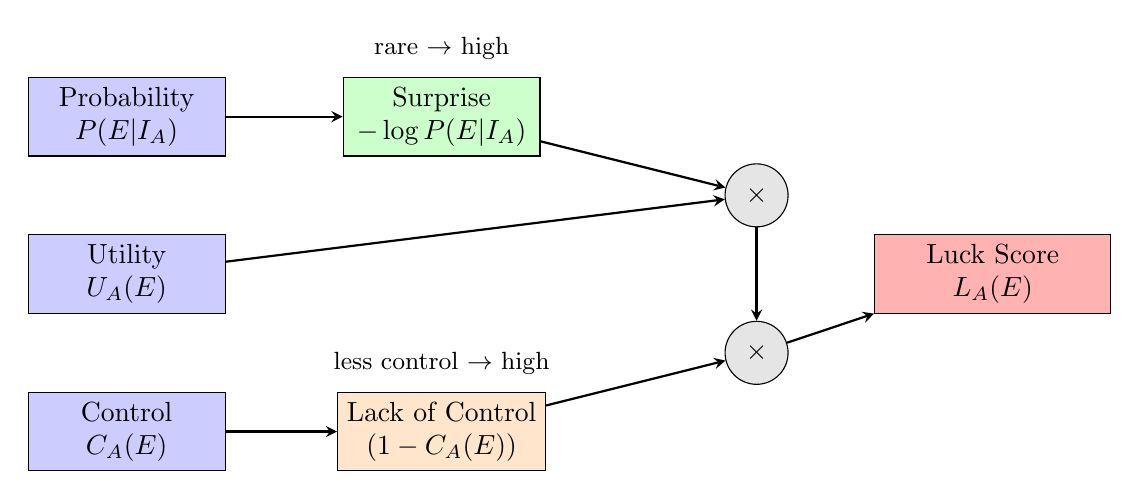
\begin{tikzpicture}[
      component/.style={rectangle, draw, fill=blue!20, minimum width=2.5cm, minimum height=1cm, align=center},
      multiplier/.style={circle, draw, fill=gray!20, minimum size=0.8cm},
      arrow/.style={->, >=stealth, thick}
    ]
      % Three components
      \node[component] (prob) at (0,0) {Probability\\$P(E|I_A)$};
      \node[component] (util) at (0,-2) {Utility\\$U_A(E)$};
      \node[component] (ctrl) at (0,-4) {Control\\$C_A(E)$};

      % Transformations
      \node[component, fill=green!20] (surp) at (4,0) {Surprise\\$-\log P(E|I_A)$};
      \node[component, fill=orange!20] (lack) at (4,-4) {Lack of Control\\$(1-C_A(E))$};

      % Result
      \node[multiplier] (mult1) at (8,-1) {$\times$};
      \node[multiplier] (mult2) at (8,-3) {$\times$};
      \node[component, fill=red!30, minimum width=3cm] (luck) at (11,-2) {Luck Score\\$L_A(E)$};

      % Arrows
      \draw[arrow] (prob) -- (surp);
      \draw[arrow] (ctrl) -- (lack);
      \draw[arrow] (surp) -- (mult1);
      \draw[arrow] (util) -- (mult1);
      \draw[arrow] (mult1) -- (mult2);
      \draw[arrow] (lack) -- (mult2);
      \draw[arrow] (mult2) -- (luck);

      % Labels
      \node[above=0.1cm of surp, font=\small] {rare $\rightarrow$ high};
      \node[above=0.1cm of lack, font=\small] {less control $\rightarrow$ high};
    \end{tikzpicture}
    \caption{Three components of the luck function combine multiplicatively. Probability is transformed into surprise (rarer events score higher), control is inverted (less control increases luck), and utility provides value weighting.}
    \label{fig:components}
  \end{figure}

% ==============================================================================
  \subsection{Motivation for Formalization}

  Formalizing luck serves multiple purposes. In moral and political philosophy,
  it clarifies debates about desert and responsibility. If outcomes depend
  substantially on luck, claims that individuals deserve their positions
  become more difficult to sustain. In institutional design,
  understanding luck enables fairer evaluation systems that account for
  factors beyond individual control. In policy analysis, measuring the
  role of luck informs debates about taxation, social insurance, and
  equality of opportunity.

  Empirical measurement requires precise definitions. Without formal structure,
  assertions about the importance of luck remain speculative. A mathematical
  framework enables testable predictions, quantitative comparisons
  across contexts, and evidence-based policy recommendations.

% ==============================================================================
  \subsection{Related Concepts}

  Several mathematical and philosophical traditions inform this
  framework:

  \begin{itemize}
    \item \textbf{Probability Theory:} Provides the foundation for
      quantifying surprise and rare events through probability measures
      and information theory.

    \item \textbf{Decision Theory:} Supplies utility functions for
      valuing outcomes and expected utility calculations for separating
      realized outcomes from expectations.

    \item \textbf{Causal Inference:} Offers tools for identifying
      controllable versus uncontrollable factors through causal graphs
      and counterfactual reasoning.

    \item \textbf{Game Theory:} Distinguishes strategic skill from
      chance elements in mixed games of skill and luck.

    \item \textbf{Moral Philosophy:} Examines the normative implications
      of luck through analyses of moral luck and distributive justice.
  \end{itemize}

% ##############################################################################
  \section{Mathematical Framework}
  \label{sec:theory}

% ==============================================================================
  \subsection{Notation and Definitions}

  Let $\Omega$ denote a sample space of possible events, $\mathcal{F}$ a
  $\sigma$-algebra on $\Omega$, and $P$ a probability measure. An agent
  $A$ at time $t$ possesses an information set
  $I_{A}(t) \subseteq \mathcal{F}$ representing their knowledge. An event
  $E \in \mathcal{F}$ occurs with conditional probability $P(E \mid I_{A}
  (t))$.

  \begin{definition}[Agent Utility]
    A utility function $U_{A}: \mathcal{F}\to \mathbb{R}$ assigns value to
    events from the perspective of agent $A$. Positive values represent
    favorable outcomes, negative values represent unfavorable outcomes,
    and zero represents neutral events.
  \end{definition}

  \begin{definition}[Control]
    The control function $C_{A}: \mathcal{F}\to [0,1]$ measures the degree
    to which agent $A$ causally influences event $E$. $C_{A}(E) = 0$
    indicates no control (pure chance), while $C_{A}(E) = 1$ indicates complete
    control (fully determined by agent's actions).
  \end{definition}

% ==============================================================================
  \subsection{Core Luck Function}

  We define luck as a function of probability, utility, and control.

  \begin{definition}[Luck]
    \label{def:luck} The luck experienced by agent $A$ from event $E$ is:
    \begin{equation}
      L_{A}(E) = U_{A}(E) \cdot S(E \mid I_{A}) \cdot (1 - C_{A}(E))
    \end{equation}
    where $S(E \mid I_{A})$ is the surprise function measuring the
    unexpectedness of $E$ given information $I_{A}$.
  \end{definition}

  The surprise function $S$ quantifies rarity. A natural choice based on
  information theory is:
  \begin{equation}
    S(E \mid I_{A}) = -\log P(E \mid I_{A})
  \end{equation}

  \begin{figure}[h]
    \centering
    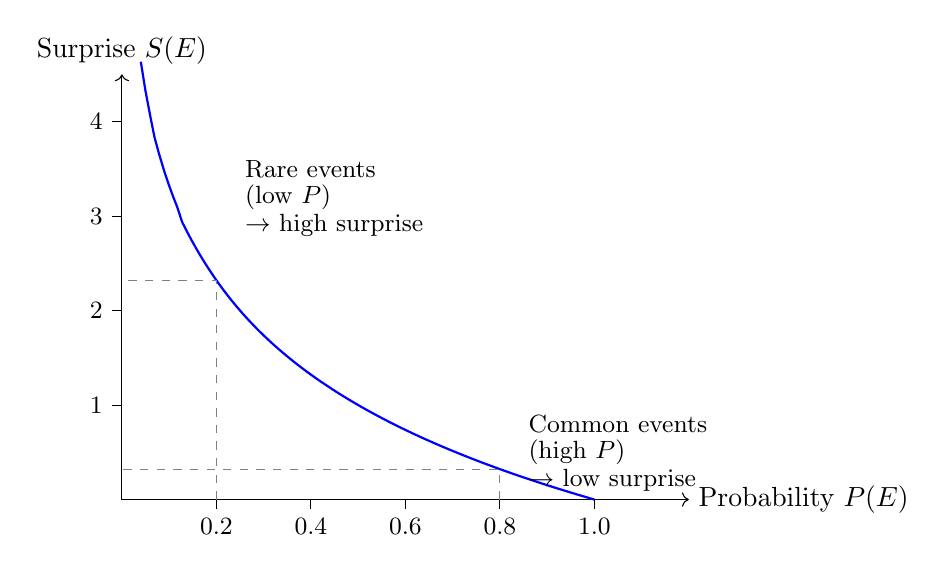
\begin{tikzpicture}[scale=1.2]
      % Axes
      \draw[->] (0,0) -- (6,0) node[right] {Probability $P(E)$};
      \draw[->] (0,0) -- (0,4.5) node[above] {Surprise $S(E)$};

      % Tick marks and labels
      \foreach \x/\label in {1/0.2, 2/0.4, 3/0.6, 4/0.8, 5/1.0} {
        \draw (\x,0) -- (\x,-0.1) node[below, font=\small] {\label};
      }
      \foreach \y/\label in {1/1, 2/2, 3/3, 4/4} {
        \draw (0,\y) -- (-0.1,\y) node[left, font=\small] {\label};
      }

      % The curve S = -ln(P) scaled appropriately
      \draw[thick, blue, domain=0.2:5, samples=100] plot ({\x}, {-ln(\x/5)/ln(2)});

      % Annotations
      \draw[dashed, gray] (1,0) -- (1,{-ln(0.2)/ln(2)}) -- (0,{-ln(0.2)/ln(2)});
      \draw[dashed, gray] (4,0) -- (4,{-ln(0.8)/ln(2)}) -- (0,{-ln(0.8)/ln(2)});

      \node[anchor=west, font=\small] at (1.2, 3.5) {Rare events};
      \node[anchor=west, font=\small] at (1.2, 3.2) {(low $P$)};
      \node[anchor=west, font=\small] at (1.2, 2.9) {$\rightarrow$ high surprise};

      \node[anchor=west, font=\small] at (4.2, 0.8) {Common events};
      \node[anchor=west, font=\small] at (4.2, 0.5) {(high $P$)};
      \node[anchor=west, font=\small] at (4.2, 0.2) {$\rightarrow$ low surprise};
    \end{tikzpicture}
    \caption{The surprise function $S(E) = -\log P(E)$ transforms probability into a rarity score. Rare events (low probability) receive high surprise scores, while common events (high probability) receive low scores. The logarithmic form ensures additivity over independent events.}
    \label{fig:surprise}
  \end{figure}

  This formulation satisfies several desirable properties:

  \begin{proposition}
    The luck function $L_{A}(E)$ is:
    \begin{enumerate}
      \item Monotonically increasing in outcome value for favorable events

      \item Monotonically decreasing in probability (rarer events are
        luckier)

      \item Monotonically decreasing in control (less controllable
        events are luckier)

      \item Zero when $U_{A}(E) = 0$ (neutral outcomes)

      \item Zero when $C_{A}(E) = 1$ (fully controlled outcomes)

      \item Information-dependent through $P(E \mid I_{A})$
    \end{enumerate}
  \end{proposition}

% ==============================================================================
  \subsection{Alternative Formulations}

  Several variants of the core luck function address different
  analytical needs.

% ------------------------------------------------------------------------------
  \subsubsection{Deviation-Based Luck}

  When repeated trials or comparable scenarios exist, luck can be
  measured as deviation from expectation:
  \begin{equation}
    L_{A}^{\text{dev}}(E) = U_{A}(E) - \mathbb{E}[U_{A}(E') \mid S_{A}]
  \end{equation}
  where $S_{A}$ represents the agent's strategy or controllable choices,
  and the expectation is taken over events $E'$ that could occur under
  that strategy. This formulation is particularly useful in skill-luck decomposition
  for repeated performance evaluation.

% ------------------------------------------------------------------------------
  \subsubsection{Fragility-Based Luck}

  Outcomes that would change under small perturbations reflect greater
  luck:
  \begin{equation}
    L_{A}^{\text{frag}}(E) = U_{A}(E) \cdot \left(1 - P(E \mid \text{perturbations}
    )\right)
  \end{equation}
  This captures near-miss scenarios where slight differences in circumstances
  would have produced substantially different outcomes.

% ------------------------------------------------------------------------------
  \subsubsection{Time-Aggregated Luck}

  For sequences of events over time $t = 1, \ldots, T$:
  \begin{equation}
    L_{A}^{T}= \sum_{t=1}^{T}\delta^{t} L_{A}(E_{t})
  \end{equation}
  where $\delta \in (0,1]$ is a temporal discount factor. This
  formulation addresses cumulative luck and path dependence in life
  trajectories.

  \begin{figure}[h]
    \centering
    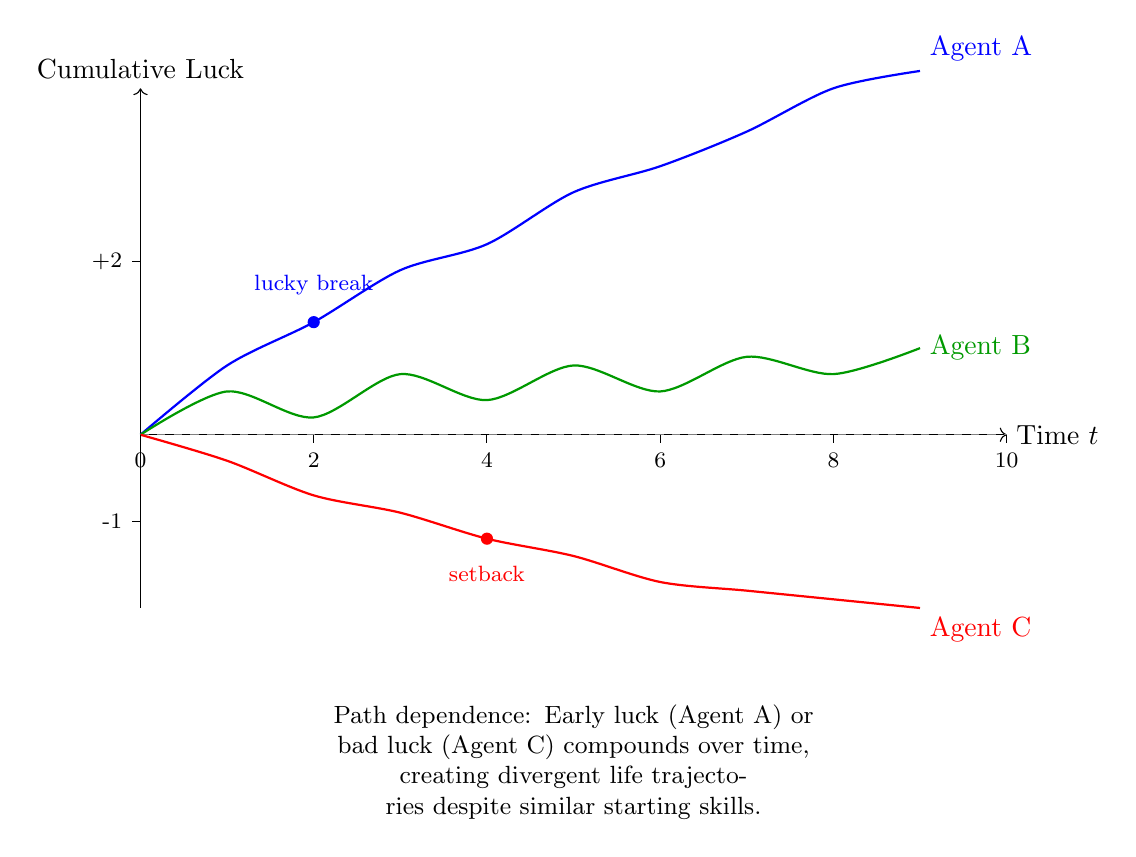
\begin{tikzpicture}[scale=1.1]
      % Axes
      \draw[->] (0,0) -- (10,0) node[right] {Time $t$};
      \draw[->] (0,-2) -- (0,4) node[above] {Cumulative Luck};
      \draw[dashed, gray] (0,0) -- (10,0);

      % Three trajectories
      % Agent A - consistently lucky
      \draw[thick, blue, smooth] plot coordinates {
        (0,0) (1,0.8) (2,1.3) (3,1.9) (4,2.2) (5,2.8) (6,3.1) (7,3.5) (8,4.0) (9,4.2)
      };
      \node[blue, above right] at (9,4.2) {Agent A};

      % Agent B - mixed luck
      \draw[thick, green!60!black, smooth] plot coordinates {
        (0,0) (1,0.5) (2,0.2) (3,0.7) (4,0.4) (5,0.8) (6,0.5) (7,0.9) (8,0.7) (9,1.0)
      };
      \node[green!60!black, right] at (9,1.0) {Agent B};

      % Agent C - consistently unlucky
      \draw[thick, red, smooth] plot coordinates {
        (0,0) (1,-0.3) (2,-0.7) (3,-0.9) (4,-1.2) (5,-1.4) (6,-1.7) (7,-1.8) (8,-1.9) (9,-2.0)
      };
      \node[red, below right] at (9,-2.0) {Agent C};

      % Key events marked
      \fill[blue] (2,1.3) circle (2pt);
      \node[blue, above, font=\footnotesize] at (2,1.5) {lucky break};
      \fill[red] (4,-1.2) circle (2pt);
      \node[red, below, font=\footnotesize] at (4,-1.4) {setback};

      % Time labels
      \foreach \x in {0,2,4,6,8,10} {
        \draw (\x,0) -- (\x,-0.1) node[below, font=\footnotesize] {\x};
      }
      \draw (0,2) -- (-0.1,2) node[left, font=\footnotesize] {+2};
      \draw (0,-1) -- (-0.1,-1) node[left, font=\footnotesize] {-1};

      % Annotation
      \node[below, text width=9cm, align=center, font=\small] at (5,-3) {
        Path dependence: Early luck (Agent A) or bad luck (Agent C) compounds over time,\\
        creating divergent life trajectories despite similar starting skills.
      };
    \end{tikzpicture}
    \caption{Time-aggregated luck trajectories for three agents. Early luck events compound over time through path dependence, leading to divergent cumulative outcomes. Agent A benefits from consistent positive luck that creates opportunities for further success. Agent C faces compounding disadvantage from early setbacks. Agent B experiences mixed luck with limited cumulative effect.}
    \label{fig:trajectories}
  \end{figure}

% ==============================================================================
  \subsection{Skill-Luck Decomposition}

  Observed outcomes $Y$ can be decomposed into skill and luck components.
  Let $S_{A}$ denote the agent's strategy space and $R$ denote random
  variables outside the agent's control.

  \begin{definition}[Expected Performance]
    The skill-based expected outcome is:
    \begin{equation}
      \bar{Y}_{A} = \mathbb{E}[Y \mid S_{A}, I_{A}]
    \end{equation}
  \end{definition}

  \begin{definition}[Luck Component]
    The luck component of outcome $Y$ is:
    \begin{equation}
      L_{A}(Y) = Y - \bar{Y}_{A}
    \end{equation}
  \end{definition}

  This decomposition enables performance evaluation that accounts for
  uncontrollable factors. In contexts with repeated observations, the
  variance of outcomes can be partitioned:
  \begin{equation}
    \text{Var}(Y) = \text{Var}(\bar{Y}_{A}) + \text{Var}(L_{A}(Y))
  \end{equation}
  where $\text{Var}(\bar{Y}_{A})$ represents skill-based variation and $\text{Var}
  (L_{A}(Y))$ represents luck-based variation.

  \begin{figure}[h]
    \centering
    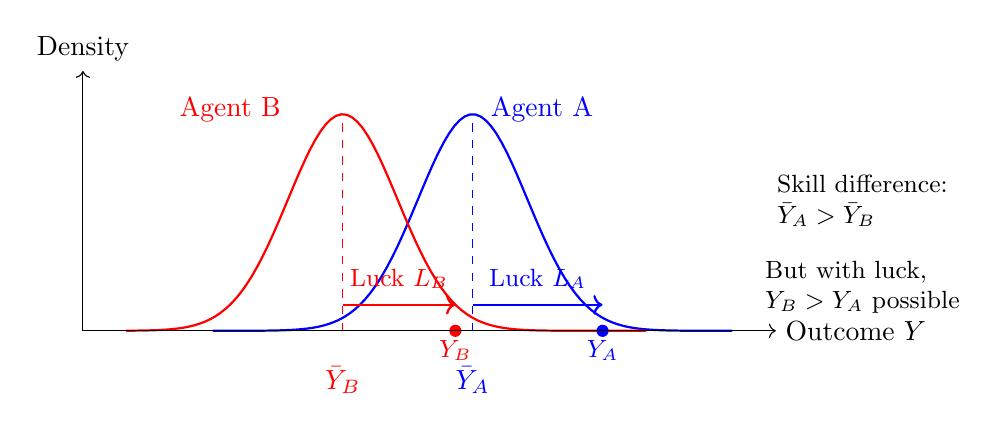
\begin{tikzpicture}[scale=1.1]
      % Draw normal distribution curves
      % Agent A - higher skill
      \draw[thick, blue, domain=-2:4, samples=100] plot ({\x}, {2.5*exp(-(\x-1)^2/0.8)});
      \draw[dashed, blue] (1,0) -- (1,2.5);
      \node[blue, below] at (1,-0.3) {$\bar{Y}_A$};
      \node[blue, above] at (1.8,2.3) {Agent A};

      % Agent B - lower skill
      \draw[thick, red, domain=-3:3, samples=100] plot ({\x}, {2.5*exp(-(\x+0.5)^2/0.8)});
      \draw[dashed, red] (-0.5,0) -- (-0.5,2.5);
      \node[red, below] at (-0.5,-0.3) {$\bar{Y}_B$};
      \node[red, above] at (-1.8,2.3) {Agent B};

      % Actual outcomes
      \draw[->, thick, blue] (1,0.3) -- (2.5,0.3);
      \node[blue, font=\small] at (1.75, 0.6) {Luck $L_A$};
      \fill[blue] (2.5,0) circle (2pt) node[below, font=\small] {$Y_A$};

      \draw[->, thick, red] (-0.5,0.3) -- (0.8,0.3);
      \node[red, font=\small] at (0.15, 0.6) {Luck $L_B$};
      \fill[red] (0.8,0) circle (2pt) node[below, font=\small] {$Y_B$};

      % Axes
      \draw[->] (-3.5,0) -- (4.5,0) node[right] {Outcome $Y$};
      \draw[->] (-3.5,0) -- (-3.5,3) node[above] {Density};

      % Annotation
      \node[align=left, font=\small] at (5.5, 1.5) {Skill difference:\\$\bar{Y}_A > \bar{Y}_B$};
      \node[align=left, font=\small] at (5.5, 0.5) {But with luck,\\$Y_B > Y_A$ possible};
    \end{tikzpicture}
    \caption{Skill-luck decomposition for two agents. Expected outcomes $\bar{Y}_A$ and $\bar{Y}_B$ reflect skill differences. Actual outcomes $Y_A$ and $Y_B$ deviate due to luck. Agent B with lower skill can outperform Agent A through favorable luck, though this becomes less likely as skill differences increase.}
    \label{fig:decomposition}
  \end{figure}

% ==============================================================================
  \subsection{Axioms and Properties}

  The framework rests on several axioms that formalize intuitive
  properties of luck:

  \begin{assumption}
    [Neutrality] Outcomes with zero utility contribute zero luck:
    $U_{A}(E) = 0 \implies L_{A}(E) = 0$.
  \end{assumption}

  \begin{assumption}
    [Control Dominance] Fully controlled outcomes are not lucky:
    $C_{A}(E) = 1 \implies L_{A}(E) = 0$.
  \end{assumption}

  \begin{assumption}
    [Information Dependence] Luck depends on the agent's prior information:
    $L_{A}(E)$ is a function of $P(E \mid I_{A})$ rather than $P(E)$
    alone.
  \end{assumption}

  \begin{assumption}
    [Value Monotonicity] For events with equal probability and control,
    luck increases with absolute utility: if $P(E_{1} \mid I_{A}) = P(E_{2}
    \mid I_{A})$ and $C_{A}(E_{1}) = C_{A}(E_{2})$, then
    $|L_{A}(E_{1})| < |L_{A}(E_{2})|$ when
    $|U_{A}(E_{1})| < |U_{A}(E_{2})|$.
  \end{assumption}

% ##############################################################################
  \section{Event Rating and Measurement}
  \label{sec:rating}

% ==============================================================================
  \subsection{Rating Pipeline}

  Practical application of the framework requires a systematic procedure
  for rating events. We propose a step-by-step pipeline:

  \begin{figure}[h]
    \centering
    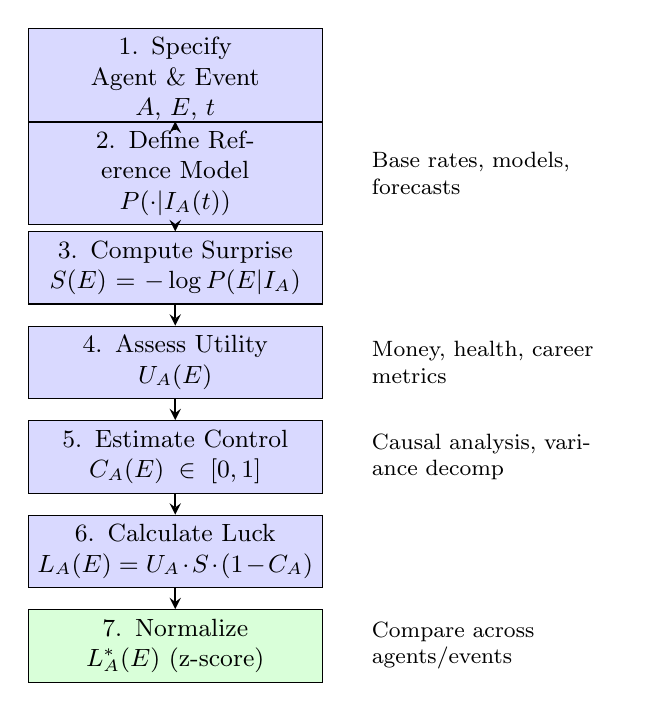
\begin{tikzpicture}[
      node distance=1.2cm,
      stepnode/.style={rectangle, draw, fill=blue!15, text width=3.5cm, minimum height=0.9cm, align=center, font=\small},
      decision/.style={diamond, draw, fill=orange!15, text width=2cm, minimum height=0.8cm, align=center, font=\small},
      arrow/.style={->, >=stealth, thick}
    ]
      % Steps
      \node[stepnode] (step1) {1. Specify Agent \& Event\\$A$, $E$, $t$};
      \node[stepnode, below of=step1] (step2) {2. Define Reference Model\\$P(\cdot|I_A(t))$};
      \node[stepnode, below of=step2] (step3) {3. Compute Surprise\\$S(E) = -\log P(E|I_A)$};
      \node[stepnode, below of=step3] (step4) {4. Assess Utility\\$U_A(E)$};
      \node[stepnode, below of=step4] (step5) {5. Estimate Control\\$C_A(E) \in [0,1]$};
      \node[stepnode, below of=step5] (step6) {6. Calculate Luck\\$L_A(E) = U_A \cdot S \cdot (1-C_A)$};
      \node[stepnode, below of=step6, fill=green!15] (step7) {7. Normalize\\$L_A^*(E)$ (z-score)};

      % Arrows
      \draw[arrow] (step1) -- (step2);
      \draw[arrow] (step2) -- (step3);
      \draw[arrow] (step3) -- (step4);
      \draw[arrow] (step4) -- (step5);
      \draw[arrow] (step5) -- (step6);
      \draw[arrow] (step6) -- (step7);

      % Side annotations
      \node[right=0.5cm of step2, text width=3cm, font=\footnotesize, align=left] {Base rates, models, forecasts};
      \node[right=0.5cm of step4, text width=3cm, font=\footnotesize, align=left] {Money, health, career metrics};
      \node[right=0.5cm of step5, text width=3cm, font=\footnotesize, align=left] {Causal analysis, variance decomp};
      \node[right=0.5cm of step7, text width=3cm, font=\footnotesize, align=left] {Compare across agents/events};
    \end{tikzpicture}
    \caption{Event rating pipeline. The seven-step procedure transforms raw event information into a normalized luck score suitable for cross-agent and cross-event comparison.}
    \label{fig:pipeline}
  \end{figure}

% ------------------------------------------------------------------------------
  \subsubsection{Step 1: Specify Agent and Event}

  Clearly identify the agent $A$, the event $E$, and the time $t$ at
  which the event occurs. Luck is agent-relative and context-dependent.

% ------------------------------------------------------------------------------
  \subsubsection{Step 2: Define Reference Model}

  Construct a probability model $P(\cdot \mid I_{A}(t))$ representing
  the agent's information state prior to the event. This may involve:
  \begin{itemize}
    \item Historical base rates for similar events

    \item Statistical models fitted to relevant data

    \item Expert forecasts or prediction markets

    \item Agent-specific models accounting for their knowledge and position
  \end{itemize}

% ------------------------------------------------------------------------------
  \subsubsection{Step 3: Compute Surprise}

  Calculate the surprise score:
  \begin{equation}
    S(E) = -\log P(E \mid I_{A})
  \end{equation}
  Low-probability events receive higher surprise scores.

% ------------------------------------------------------------------------------
  \subsubsection{Step 4: Assess Outcome Value}

  Determine utility $U_{A}(E)$ using appropriate scales:
  \begin{itemize}
    \item Monetary value for financial outcomes

    \item Health metrics (life expectancy, quality-adjusted life years)
      for health outcomes

    \item Career advancement measures for professional outcomes

    \item Normalized scores for comparative analysis
  \end{itemize}

% ------------------------------------------------------------------------------
  \subsubsection{Step 5: Estimate Control}

  Quantify the degree of agent control $C_{A}(E) \in [0,1]$. Methods
  include:
  \begin{itemize}
    \item Causal modeling to identify controllable versus uncontrollable
      factors

    \item Variance decomposition showing proportion explained by agent's
      actions

    \item Counterfactual analysis examining outcome sensitivity to agent's
      choices

    \item Repeatability analysis measuring consistency of outcomes across
      similar scenarios
  \end{itemize}

% ------------------------------------------------------------------------------
  \subsubsection{Step 6: Calculate Luck Score}

  Apply the luck function:
  \begin{equation}
    L_{A}(E) = U_{A}(E) \cdot S(E) \cdot (1 - C_{A}(E))
  \end{equation}

% ------------------------------------------------------------------------------
  \subsubsection{Step 7: Normalize}

  For cross-event or cross-agent comparison, normalize within relevant populations:
  \begin{equation}
    L_{A}^{*}(E) = \frac{L_{A}(E) - \mu_{L}}{\sigma_{L}}
  \end{equation}
  producing a standardized luck z-score.

% ==============================================================================
  \subsection{Data Requirements}

  Empirical application requires several types of data:

  \begin{table}[H]
    \centering
    \begin{tabular}{ll}
      \toprule \textbf{Data Type} & \textbf{Purpose}               \\
      \midrule Probability data   & Estimate $P(E \mid I_{A})$     \\
      Historical frequencies      & Base rates for similar events  \\
      Information records         & Define information set $I_{A}$ \\
      Outcome measurements        & Quantify utility $U_{A}(E)$    \\
      Decision logs               & Track controllable actions     \\
      Causal data                 & Estimate control $C_{A}(E)$    \\
      Baseline performance        & Compute expected values        \\
      Population distributions    & Normalize luck scores          \\
      \bottomrule
    \end{tabular}
    \caption{Data requirements for empirical luck measurement}
    \label{tab:data}
  \end{table}

% ==============================================================================
  \subsection{Example Application}

  Consider a concrete example: an entrepreneur's startup succeeds after
  raising venture capital. We analyze the luck component:

  \begin{itemize}
    \item \textbf{Event:} Startup achieves successful exit within five
      years

    \item \textbf{Probability:} Base rate for similar ventures is
      approximately 10\%, so $P(E) = 0.1$ and
      $S(E) = -\log(0.1) \approx 2.3$

    \item \textbf{Utility:} Financial gain of \$5M, normalized to
      $U_{A}(E) = 5$

    \item \textbf{Control:} Entrepreneur's strategy and execution
      contributed substantially, but market conditions and network effects
      were also crucial; estimate $C_{A}(E) = 0.6$

    \item \textbf{Luck Score:}
      $L_{A}(E) = 5 \times 2.3 \times (1 - 0.6) = 4.6$
  \end{itemize}

  This positive luck score indicates that while the entrepreneur's skill
  was important, favorable circumstances and timing contributed significantly
  to the outcome.

  \begin{figure}[h]
    \centering
    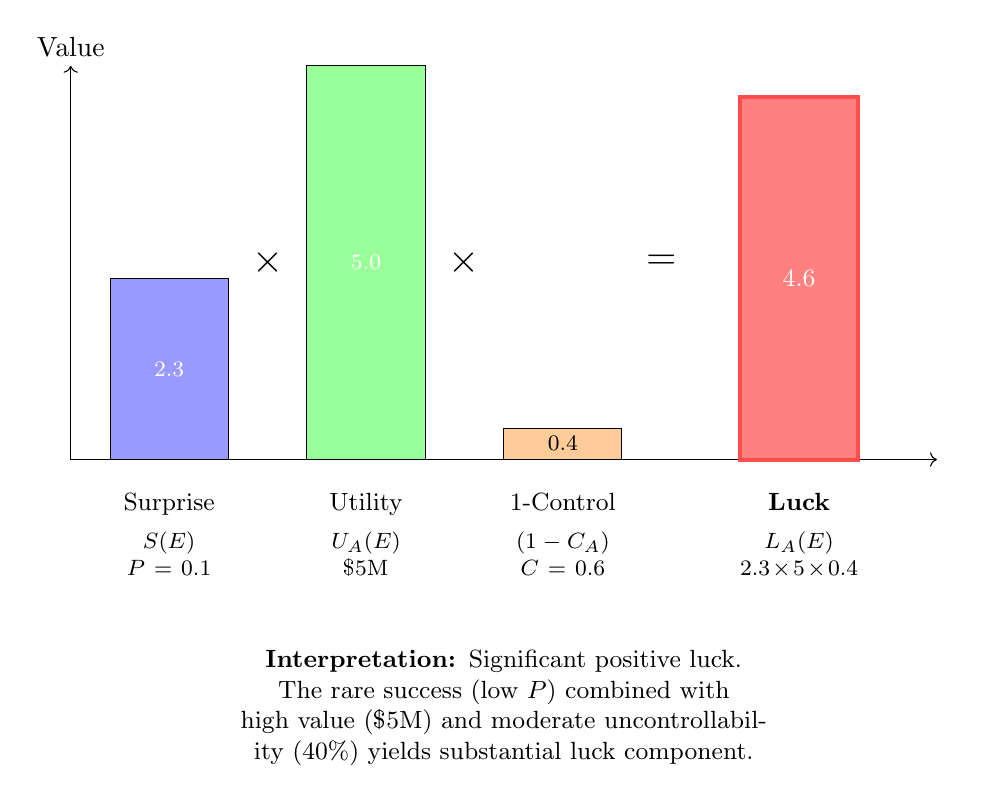
\begin{tikzpicture}[scale=1.0]
      % Bar chart
      \draw[->] (0,0) -- (0,5) node[above] {Value};
      \draw[->] (0,0) -- (11,0) node[right] {};

      % Bars
      % Probability/Surprise
      \draw[fill=blue!40] (0.5,0) rectangle (2,2.3) node[midway, white, font=\footnotesize] {2.3};
      \node[below, font=\small] at (1.25,-0.3) {Surprise};
      \node[below, font=\footnotesize, text width=1.5cm, align=center] at (1.25,-0.8) {$S(E)$\\$P=0.1$};

      % Utility
      \draw[fill=green!40] (3,0) rectangle (4.5,5) node[midway, white, font=\footnotesize] {5.0};
      \node[below, font=\small] at (3.75,-0.3) {Utility};
      \node[below, font=\footnotesize, text width=1.5cm, align=center] at (3.75,-0.8) {$U_A(E)$\\\$5M};

      % Control
      \draw[fill=orange!40] (5.5,0) rectangle (7,0.4) node[midway, font=\footnotesize] {0.4};
      \node[below, font=\small] at (6.25,-0.3) {1-Control};
      \node[below, font=\footnotesize, text width=1.5cm, align=center] at (6.25,-0.8) {$(1-C_A)$\\$C=0.6$};

      % Result
      \draw[fill=red!50, draw=red!70, line width=1.5pt] (8.5,0) rectangle (10,4.6);
      \node[white, font=\small] at (9.25,2.3) {4.6};
      \node[below, font=\small] at (9.25,-0.3) {\textbf{Luck}};
      \node[below, font=\footnotesize, text width=1.5cm, align=center] at (9.25,-0.8) {$L_A(E)$\\$2.3 \times 5 \times 0.4$};

      % Multiplication signs
      \node[font=\Large] at (2.5,2.5) {$\times$};
      \node[font=\Large] at (5,2.5) {$\times$};
      \node[font=\Large] at (7.5,2.5) {$=$};

      % Interpretation
      \node[below, text width=10cm, align=center, font=\small] at (5.5,-2.3) {
        \textbf{Interpretation:} Significant positive luck. The rare success (low $P$) combined with\\
        high value (\$5M) and moderate uncontrollability (40\%) yields substantial luck component.
      };
    \end{tikzpicture}
    \caption{Startup example calculation. The entrepreneur's success is decomposed into components: surprise from low base rate ($P=0.1$), high financial utility (\$5M normalized to 5), and moderate lack of control (0.4, since skill $C=0.6$ was important). The resulting luck score of 4.6 indicates substantial favorable luck.}
    \label{fig:example}
  \end{figure}

% ##############################################################################
  \section{Societal Modeling and Aggregate Measures}
  \label{sec:society}

% ==============================================================================
  \subsection{Modeling Life Outcomes}

  To analyze luck at the societal level, we model individual life
  outcomes as a function of three input categories:

  \begin{itemize}
    \item \textbf{Circumstances} $B_{i}$: Factors not chosen by the individual
      (parental background, birth location, cohort, genetics)

    \item \textbf{Choices} $A_{i}$: Factors under individual control (effort,
      decisions, strategies)

    \item \textbf{Shocks} $S_{i}$: Random events affecting the individual
      (accidents, encounters, policy changes)
  \end{itemize}

  A general outcome model takes the form:
  \begin{equation}
    Y_{i} = f(B_{i}, A_{i}) + g(S_{i}) + \varepsilon_{i}
  \end{equation}
  where $f$ represents the deterministic relationship between
  circumstances, choices, and outcomes, $g$ captures the effect of random
  shocks, and $\varepsilon_{i}$ represents measurement error or small
  unmodeled factors.

  \begin{figure}[h]
    \centering
    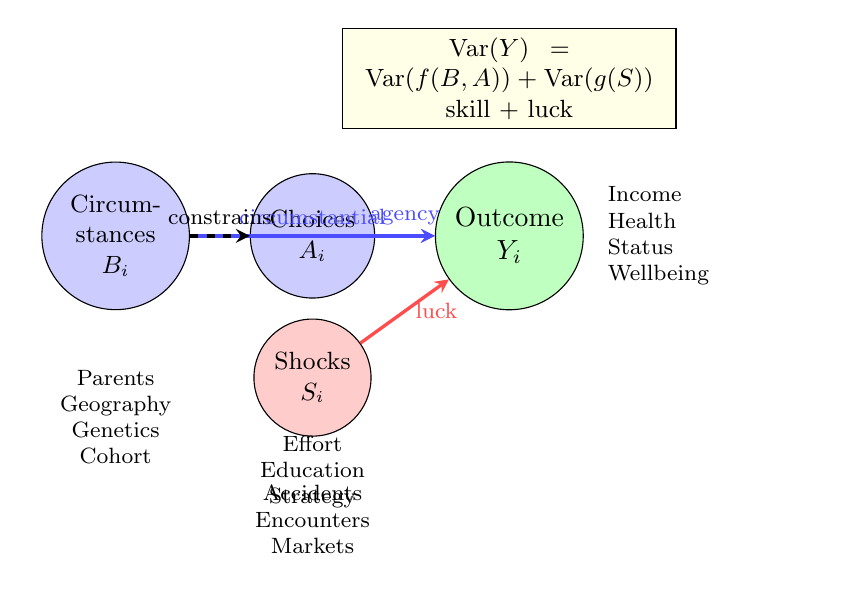
\begin{tikzpicture}[
      node distance=2.5cm and 2cm,
      varnode/.style={circle, draw, fill=blue!20, minimum size=1.3cm, align=center, font=\small},
      outcome/.style={circle, draw, fill=green!25, minimum size=1.5cm, align=center, font=\normalsize},
      shock/.style={circle, draw, fill=red!20, minimum size=1.3cm, align=center, font=\small},
      arrow/.style={->, >=stealth, very thick}
    ]
      % Nodes
      \node[varnode] (B) {Circum-\\stances\\$B_i$};
      \node[varnode, right of=B] (A) {Choices\\$A_i$};
      \node[shock, below of=A, node distance=1.8cm] (S) {Shocks\\$S_i$};
      \node[outcome, right of=A] (Y) {Outcome\\$Y_i$};

      % Arrows
      \draw[arrow, blue!70] (B) -- (Y) node[midway, above, font=\footnotesize] {circumstantial};
      \draw[arrow, blue!70] (A) -- (Y) node[midway, above, font=\footnotesize] {agency};
      \draw[arrow, red!70] (S) -- (Y) node[midway, right, font=\footnotesize] {luck};
      \draw[arrow, dashed] (B) -- (A) node[midway, above, font=\footnotesize] {constrains};

      % Annotations
      \node[below of=B, node distance=2.3cm, text width=2cm, align=center, font=\footnotesize] {Parents\\Geography\\Genetics\\Cohort};
      \node[below of=A, node distance=3cm, text width=2cm, align=center, font=\footnotesize] {Effort\\Education\\Strategy};
      \node[below of=S, node distance=1.8cm, text width=2cm, align=center, font=\footnotesize] {Accidents\\Encounters\\Markets};
      \node[right of=Y, node distance=2.5cm, text width=2.5cm, align=left, font=\footnotesize] {Income\\Health\\Status\\Wellbeing};

      % Variance decomposition annotation
      \node[above of=Y, node distance=2cm, text width=4cm, align=center, font=\small, draw, fill=yellow!10] {
        $\text{Var}(Y) = \text{Var}(f(B,A)) + \text{Var}(g(S))$\\
        skill + luck
      };
    \end{tikzpicture}
    \caption{Causal model of societal outcomes. Circumstances $B_i$ (unearned advantages) and choices $A_i$ (agency) jointly determine expected outcomes, while shocks $S_i$ (random events) introduce luck. Circumstances also constrain available choices. The variance decomposition separates skill-based from luck-based variation in outcomes.}
    \label{fig:causal}
  \end{figure}

% ==============================================================================
  \subsection{Individual Luck Measures}

  Three complementary measures capture different aspects of luck:

% ------------------------------------------------------------------------------
  \subsubsection{Residual Luck}

  Residual luck measures the deviation of actual outcomes from
  predictions based on circumstances and choices:
  \begin{equation}
    L_{i}^{\text{res}}= Y_{i} - \mathbb{E}[Y_{i} \mid B_{i}, A_{i}]
  \end{equation}
  This represents the core luck component—the portion of outcomes not explained
  by observable inputs.

% ------------------------------------------------------------------------------
  \subsubsection{Surprise-Weighted Luck}

  For outcomes far from expectations, surprise weighting emphasizes extreme
  cases:
  \begin{equation}
    L_{i}^{\text{sur}}= U(Y_{i}) \cdot \left[-\log P(Y_{i} \mid B_{i}, A_{i}
    )\right]
  \end{equation}

% ------------------------------------------------------------------------------
  \subsubsection{Control-Adjusted Luck}

  When control varies across individuals or contexts:
  \begin{equation}
    L_{i}^{\text{ctrl}}= (Y_{i} - \mathbb{E}[Y_{i} \mid B_{i}, A_{i}]) \cdot
    (1 - C_{i})
  \end{equation}
  where $C_{i}$ represents the degree of control individual $i$ has over
  their outcomes.

% ==============================================================================
  \subsection{Aggregate Luck Metrics}

  Societal-level analysis aggregates individual luck scores to
  characterize distributional properties.

% ------------------------------------------------------------------------------
  \subsubsection{Luck Inequality}

  The Gini coefficient of absolute luck values measures dispersion:
  \begin{equation}
    G_{L} = \frac{\sum_{i=1}^{n}\sum_{j=1}^{n}|L_{i} - L_{j}|}{2n^{2}\bar{L}}
  \end{equation}
  High luck inequality indicates that some individuals experience far
  more favorable or unfavorable luck than others.

% ------------------------------------------------------------------------------
  \subsubsection{Circumstantial Dependence}

  The proportion of outcome variance explained by circumstances (rather
  than choices or luck) measures the degree to which outcomes are predetermined
  by birth:
  \begin{equation}
    \rho_{B} = \frac{\text{Var}(\mathbb{E}[Y \mid B])}{\text{Var}(Y)}
  \end{equation}
  Higher values indicate less social mobility and greater importance of
  circumstantial luck.

% ------------------------------------------------------------------------------
  \subsubsection{Agency Contribution}

  The additional variance explained by choices beyond circumstances:
  \begin{equation}
    \rho_{A} = \frac{\text{Var}(\mathbb{E}[Y \mid B, A]) - \text{Var}(\mathbb{E}[Y
    \mid B])}{\text{Var}(Y)}
  \end{equation}
  This measures the role of individual agency in determining outcomes.

% ------------------------------------------------------------------------------
  \subsubsection{Mobility Index}

  Intergenerational mobility can be measured through the correlation between
  parent and child outcomes:
  \begin{equation}
    M = 1 - \text{Corr}(Y_{\text{parent}}, Y_{\text{child}})
  \end{equation}
  Lower correlation (higher $M$) suggests that circumstances of birth
  have less influence on eventual outcomes.

% ==============================================================================
  \subsection{Empirical Estimation}

  Practical estimation typically proceeds through regression-based variance
  decomposition. Consider a model:
  \begin{equation}
    Y_{i} = \alpha + \beta_{B} B_{i} + \beta_{A} A_{i} + \varepsilon_{i}
  \end{equation}

  Stepwise regression allows decomposition:
  \begin{enumerate}
    \item Regress $Y$ on $B$ alone: variance explained is $R^{2}_{B}$

    \item Regress $Y$ on both $B$ and $A$: variance explained is
      $R^{2}_{B,A}$

    \item Residual variance: $1 - R^{2}_{B,A}$ represents luck

    \item Agency contribution: $R^{2}_{B,A}- R^{2}_{B}$
  \end{enumerate}

  \begin{figure}[h]
    \centering
    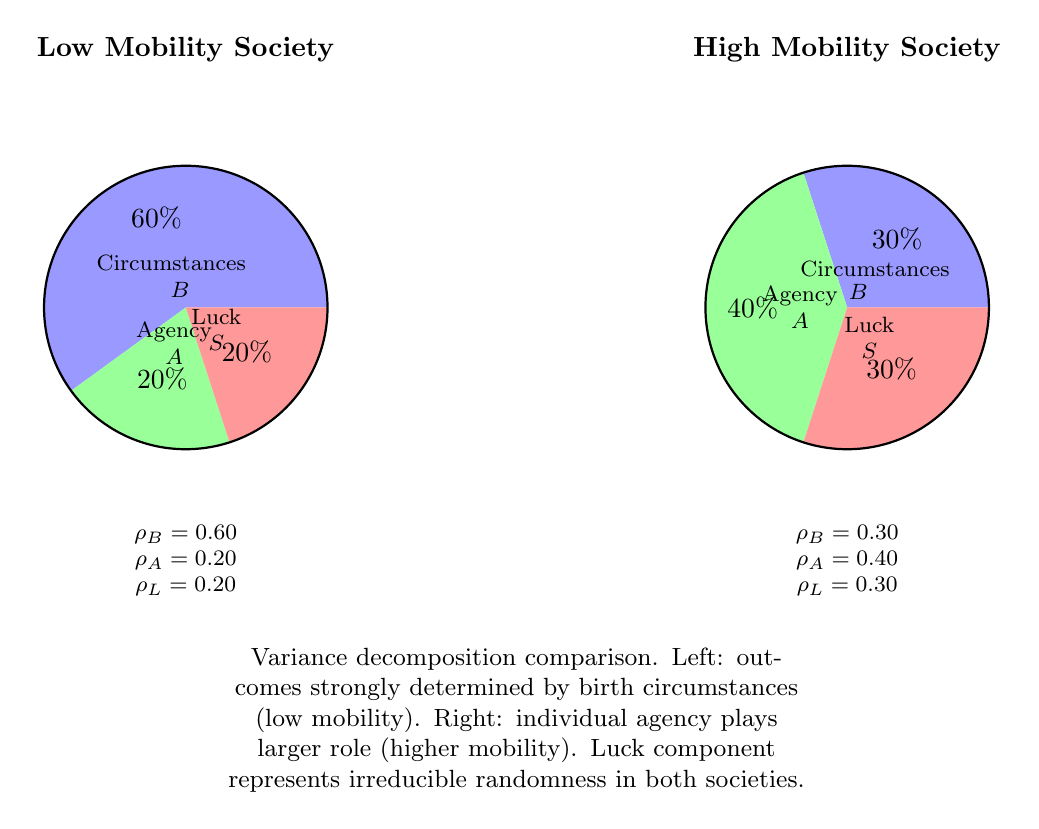
\begin{tikzpicture}[scale=1.2]
      % Two pie charts comparing societies

      % Society 1 - High circumstantial dependence
      \begin{scope}[xshift=0cm]
        \node[above] at (0,2.5) {\textbf{Low Mobility Society}};

        % Pie chart
        \fill[blue!40] (0,0) -- (0:1.5) arc (0:216:1.5) -- cycle;
        \fill[green!40] (0,0) -- (216:1.5) arc (216:288:1.5) -- cycle;
        \fill[red!40] (0,0) -- (288:1.5) arc (288:360:1.5) -- cycle;

        \draw[thick] (0,0) circle (1.5);

        % Labels with percentages
        \node at (108:1) {60\%};
        \node[font=\footnotesize] at (108:0.5) {Circumstances};
        \node[font=\footnotesize] at (108:0.2) {$B$};

        \node at (252:0.8) {20\%};
        \node[font=\footnotesize, text width=1.5cm, align=center] at (252:0.4) {Agency\\$A$};

        \node at (324:0.8) {20\%};
        \node[font=\footnotesize, text width=1.2cm, align=center] at (324:0.4) {Luck\\$S$};

        % Metrics below
        \node[below, align=center, font=\footnotesize] at (0,-2.2) {
          $\rho_B = 0.60$\\
          $\rho_A = 0.20$\\
          $\rho_L = 0.20$
        };
      \end{scope}

      % Society 2 - More mobility
      \begin{scope}[xshift=7cm]
        \node[above] at (0,2.5) {\textbf{High Mobility Society}};

        % Pie chart
        \fill[blue!40] (0,0) -- (0:1.5) arc (0:108:1.5) -- cycle;
        \fill[green!40] (0,0) -- (108:1.5) arc (108:252:1.5) -- cycle;
        \fill[red!40] (0,0) -- (252:1.5) arc (252:360:1.5) -- cycle;

        \draw[thick] (0,0) circle (1.5);

        % Labels with percentages
        \node at (54:0.9) {30\%};
        \node[font=\footnotesize] at (54:0.5) {Circumstances};
        \node[font=\footnotesize] at (54:0.2) {$B$};

        \node at (180:1) {40\%};
        \node[font=\footnotesize, text width=1.5cm, align=center] at (180:0.5) {Agency\\$A$};

        \node at (306:0.8) {30\%};
        \node[font=\footnotesize, text width=1.2cm, align=center] at (306:0.4) {Luck\\$S$};

        % Metrics below
        \node[below, align=center, font=\footnotesize] at (0,-2.2) {
          $\rho_B = 0.30$\\
          $\rho_A = 0.40$\\
          $\rho_L = 0.30$
        };
      \end{scope}

      % Legend
      \node[below, text width=12cm, align=center, font=\small] at (3.5,-3.5) {
        Variance decomposition comparison. Left: outcomes strongly determined by birth circumstances\\
        (low mobility). Right: individual agency plays larger role (higher mobility). Luck component\\
        represents irreducible randomness in both societies.
      };
    \end{tikzpicture}
    \caption{Variance decomposition in two stylized societies. The low mobility society (left) shows outcome variance dominated by circumstances of birth ($\rho_B = 0.60$), with limited role for agency ($\rho_A = 0.20$). The high mobility society (right) exhibits lower circumstantial dependence ($\rho_B = 0.30$) and greater agency contribution ($\rho_A = 0.40$). Both societies contain irreducible luck components from random shocks.}
    \label{fig:variance}
  \end{figure}

% ##############################################################################
  \section{Implications and Applications}
  \label{sec:implications}

% ==============================================================================
  \subsection{Moral and Philosophical Implications}

  The framework clarifies debates about desert and responsibility. If formal
  analysis demonstrates that outcomes depend substantially on luck rather
  than controllable factors, several philosophical implications follow:

  \begin{itemize}
    \item \textbf{Desert:} Claims that individuals fully deserve their
      outcomes become difficult to sustain when luck plays a significant
      role.

    \item \textbf{Responsibility:} Moral evaluation must account for the
      limited control agents have over their circumstances and the
      events that befall them.

    \item \textbf{Dignity:} If outcomes are substantially luck-determined,
      human worth should not be closely tied to achievement.
  \end{itemize}

  These implications align with philosophical analyses of moral luck,
  which argue that factors beyond an agent's control affect our moral
  judgments inappropriately.

% ==============================================================================
  \subsection{Policy Implications}

  Quantifying the role of luck informs policy debates across multiple domains.

% ------------------------------------------------------------------------------
  \subsubsection{Taxation and Redistribution}

  When luck contributes substantially to income and wealth, the case for
  progressive taxation and redistribution strengthens. If high earners
  benefit from favorable circumstances and chance events, claims of full
  entitlement to their income weaken. Luck-adjusted taxation could
  incorporate measurements of the luck component in individual outcomes.

% ------------------------------------------------------------------------------
  \subsubsection{Social Insurance}

  Recognition that adverse outcomes often reflect bad luck rather than poor
  choices supports comprehensive social insurance. Unemployment benefits,
  healthcare access, and disability support become justified as
  protections against uncontrollable risks rather than rewards for
  underperformance.

% ------------------------------------------------------------------------------
  \subsubsection{Educational Policy}

  Measuring luck in educational outcomes can inform admission policies and
  resource allocation. If standardized test performance reflects
  substantial circumstantial luck (parental resources, school quality, neighborhood
  effects), policies that emphasize fine-grained score differences become
  less defensible. Alternative approaches such as lottery-based
  admission among qualified candidates warrant consideration.

% ==============================================================================
  \subsection{Institutional Design}

  Organizations can incorporate luck awareness in evaluation and reward systems.

% ------------------------------------------------------------------------------
  \subsubsection{Performance Evaluation}

  Corporations and public institutions that evaluate employees on
  outcomes without accounting for luck risk misattributing results. Luck-adjusted
  performance metrics provide fairer assessments by comparing actual outcomes
  to expected outcomes given circumstances and constraints.

% ------------------------------------------------------------------------------
  \subsubsection{Promotion and Selection}

  When selecting among candidates with similar qualifications, acknowledging
  that fine-grained differences may reflect luck rather than ability supports
  lottery-based selection or increased weight on diverse criteria beyond
  narrow performance measures.

% ------------------------------------------------------------------------------
  \subsubsection{Executive Compensation}

  CEO pay often reflects firm performance that depends substantially on
  market conditions and timing. Luck-adjusted compensation schemes could
  separate controllable performance from market-driven outcomes,
  reducing excessive rewards for favorable circumstances.

% ==============================================================================
  \subsection{Empirical Rankings of Activities and Occupations}

  To illustrate the framework's application, we present empirical rankings
  of common activities and occupations according to the relative importance
  of luck versus skill in determining three distinct outcomes: income,
  social status, and societal impact. These rankings demonstrate how
  the skill-luck balance varies systematically across domains and outcome
  types.

% ------------------------------------------------------------------------------
  \subsubsection{Income Rankings}

  Table~\ref{tab:income_rankings} ranks activities by the degree to which
  luck versus skill determines income outcomes. Several patterns emerge.
  At the luck-dominated extreme, lottery gambling and casino games produce
  outcomes almost entirely independent of player skill. Inheritance and
  viral fame represent pure circumstantial luck. The middle range contains
  mixed activities where skill is necessary but insufficient: acting,
  venture capital, and stock trading all require ability but outcomes
  depend heavily on timing, context, and random events. At the skill-dominated
  end, craftsmanship, medicine, and mathematics show strong skill-outcome
  relationships where ability and practice reliably improve results.

  \begin{table}[H]
    \centering
    \small
    \begin{tabular}{clll}
      \toprule
      \textbf{Rank} & \textbf{Activity / Job} & \textbf{Dominant Factor} & \textbf{Notes} \\
      \midrule
      1 & Lottery gambling & Luck & Outcomes almost entirely random \\
      2 & Casino games (slots, roulette) & Luck & Skill has negligible impact \\
      3 & Inheritance / family background & Luck & Determined before individual action \\
      4 & Viral social media fame & Luck & Timing and algorithms dominate \\
      5 & Acting / entertainment stardom & Luck-heavy & Talent necessary but not sufficient \\
      6 & Professional sports draft success & Luck-heavy & Talent + injuries + team context \\
      7 & Venture capital startup success & Luck-heavy & Market timing dominates outcomes \\
      8 & Stock picking (short-term trading) & Luck-heavy & Noise overwhelms signal short-term \\
      9 & Academic career (tenure-track) & Mixed & Skill + timing + gatekeepers \\
      10 & Corporate executive promotion & Mixed & Performance + politics + timing \\
      11 & Sales (high-variance environments) & Mixed & Skill matters but randomness large \\
      12 & Entrepreneurship (small business) & Mixed & Execution + location + shocks \\
      13 & Journalism / writing careers & Mixed & Quality + attention dynamics \\
      14 & Software startup engineering & Skill-leaning & Skill important, market still risky \\
      15 & Competitive chess / esports & Skill-leaning & Luck minimal over many games \\
      16 & Professional programming & Skill & Outcomes strongly skill-driven \\
      17 & Engineering (civil, mechanical) & Skill & Errors and successes traceable \\
      18 & Medicine (clinical practice) & Skill & High training, bounded uncertainty \\
      19 & Skilled trades (electrician, plumber) & Skill & Experience directly impacts results \\
      20 & Craftsmanship (luthier, watchmaker) & Skill & Mastery dominates outcomes \\
      21 & Mathematics / theoretical research & Skill & Luck in insight exists, but skill dominates \\
      22 & Classical music performance & Skill & Precision and training decisive \\
      \bottomrule
    \end{tabular}
    \caption{Ranking of activities by luck versus skill in determining income. Luck-dominated activities show little relationship between effort and earnings. Mixed activities require skill but exhibit high outcome variance. Skill-dominated activities show reliable skill-income relationships. Rankings assume long careers with repeated outcomes; at short timescales, luck matters more everywhere.}
    \label{tab:income_rankings}
  \end{table}

  Three key patterns emerge from income analysis. First, income is more
  luck-driven than performance in winner-take-all markets where visibility
  and timing dominate. Second, skill dominates income in regulated, credentialed,
  or craft-based professions with direct feedback loops. Third, the
  upper tail of income distributions is almost always luck-amplified:
  even in skill-based fields, the highest earners typically benefit from
  favorable circumstances beyond their control.

  Important caveats apply. These rankings assume many trials (long careers,
  repeated outcomes). At short timescales, luck matters more in almost
  all domains. Institutions can amplify or suppress luck through safety
  nets, progressive taxation, or tournament structures. Individual cases
  within any category will vary.

% ------------------------------------------------------------------------------
  \subsubsection{Status Rankings}

  Table~\ref{tab:status_rankings} ranks activities by luck versus skill
  in determining social status. Status shows greater luck-sensitivity
  than income. Visibility and narrative dynamics dominate over contribution.
  Royalty and celebrity status are almost entirely luck-determined, assigned
  by birth or attention cascades. Even at the skill end, status depends
  substantially on recognition mechanisms, institutional prestige, and
  social networks—factors only partially controllable by individuals.

  \begin{table}[H]
    \centering
    \small
    \begin{tabular}{clll}
      \toprule
      \textbf{Rank} & \textbf{Activity / Role} & \textbf{Status Driver} & \textbf{Notes} \\
      \midrule
      1 & Royalty / inherited aristocracy & Luck & Status assigned at birth \\
      2 & Celebrity by viral exposure & Luck-heavy & Attention cascades dominate \\
      3 & Influencer / public figure (online) & Luck-heavy & Algorithms and timing crucial \\
      4 & Entertainment stardom & Luck-heavy & Winner-take-all recognition \\
      5 & Elite professional athlete & Luck-heavy & Skill required, exposure uneven \\
      6 & Billionaire entrepreneur & Luck-heavy & Extreme skew in recognition \\
      7 & Top political leader & Mixed & Skill + timing + coalition luck \\
      8 & Corporate CEO (major firm) & Mixed & Networks and succession timing \\
      9 & Prestigious academic (elite institutions) & Mixed & Reputation dynamics matter \\
      10 & Renowned artist / author & Mixed & Skill filtered by cultural luck \\
      11 & Judge / senior civil servant & Skill-leaning & Credentialed legitimacy \\
      12 & Senior physician & Skill-leaning & Status tied to expertise \\
      13 & Lawyer (high standing) & Skill-leaning & Reputation grows with competence \\
      14 & University professor & Skill-leaning & Long-run skill signal \\
      15 & Engineer (senior / chartered) & Skill & Respect tied to reliability \\
      16 & Architect & Skill & Skill and judgment visible \\
      17 & Skilled trades master & Skill & Local reputation-based status \\
      18 & Scientist (non-celebrity) & Skill & Recognition tracks contribution \\
      19 & Teacher (experienced) & Skill & Status from trust and service \\
      20 & Craftsperson & Skill & Mastery-based respect \\
      \bottomrule
    \end{tabular}
    \caption{Ranking of activities by luck versus skill in determining social status. Status proves more luck-sensitive than income, with visibility and narrative dynamics dominating contribution. Winner-take-all attention markets amplify small random differences into large status gaps. Even skill-based status depends on recognition mechanisms partially beyond individual control.}
    \label{tab:status_rankings}
  \end{table}

  The status rankings reveal that recognition mechanisms introduce substantial
  luck even when underlying performance is skill-based. Winner-take-all
  dynamics amplify small random differences—an early break, fortuitous
  timing, or algorithmic promotion—into large status disparities. Media
  visibility, institutional prestige, and network effects create path
  dependence where initial luck compounds over time.

% ------------------------------------------------------------------------------
  \subsubsection{Impact Rankings}

  Table~\ref{tab:impact_rankings} ranks activities by luck versus skill
  in producing societal impact. Interestingly, sustained impact correlates
  more strongly with skill than either income or status. Viral content
  creators achieve visibility without lasting effect. Celebrity activism
  leverages platforms but often lacks depth. In contrast, physicians,
  educators, engineers, and public health officials produce measurable,
  cumulative benefits through skill application over time.

  \begin{table}[H]
    \centering
    \small
    \begin{tabular}{clll}
      \toprule
      \textbf{Rank} & \textbf{Activity / Role} & \textbf{Impact Driver} & \textbf{Notes} \\
      \midrule
      1 & Viral content creator & Luck & Impact unpredictable, fleeting \\
      2 & Celebrity activism & Luck-heavy & Platform matters more than depth \\
      3 & Speculative finance & Luck-heavy & Impact often indirect or neutral \\
      4 & Political leader (short tenure) & Luck-heavy & Context dominates effectiveness \\
      5 & Startup founder (median outcome) & Mixed & Few high-impact successes \\
      6 & Journalist (agenda-setting roles) & Mixed & Skill + institutional leverage \\
      7 & Policy-maker / regulator & Mixed & Skill filtered through politics \\
      8 & Senior corporate executive & Mixed & Impact depends on firm context \\
      9 & NGO leader & Skill-leaning & Execution and governance matter \\
      10 & Urban planner & Skill-leaning & Long-term structural effects \\
      11 & Public health official & Skill-leaning & Expertise strongly affects outcomes \\
      12 & Physician & Skill-leaning & Direct, measurable human impact \\
      13 & Engineer (infrastructure) & Skill & Safety and reliability critical \\
      14 & Scientist (applied research) & Skill & Knowledge accumulation \\
      15 & Educator (systemic reach) & Skill & Compounding long-term effects \\
      16 & Software engineer (widely used systems) & Skill & Scalable, repeatable impact \\
      17 & Environmental scientist & Skill & Policy-relevant evidence \\
      18 & Civil servant (operational roles) & Skill & Consistent service delivery \\
      19 & Skilled trades (utilities, safety) & Skill & Quiet but essential impact \\
      20 & Caregiver / nurse & Skill & High direct human impact \\
      \bottomrule
    \end{tabular}
    \caption{Ranking of activities by luck versus skill in producing societal impact. Sustained impact correlates more strongly with skill than income or status. High-visibility roles often produce fleeting effects, while lower-visibility professional roles create measurable, cumulative benefits. Institutions with feedback loops reduce luck's role in impact generation.}
    \label{tab:impact_rankings}
  \end{table}

  The impact rankings demonstrate a striking pattern: high-impact work
  is often low-status and exhibits low variance. Caregivers, civil servants,
  and skilled tradespeople produce consistent, essential benefits that
  accumulate reliably over careers. Institutions with feedback loops—regulatory
  oversight, professional standards, service delivery metrics—reduce luck's
  role in impact generation. In contrast, activities that produce high
  status or income through luck rarely generate sustained societal benefit.

  These rankings illustrate the framework's analytical power. By decomposing
  outcomes into skill and luck components, we can identify systematic
  patterns: winner-take-all markets amplify luck, credentialed professions
  reduce it, and sustained impact requires skill regardless of status
  or income. Such analysis informs both individual career decisions and
  institutional design aimed at aligning rewards with contributions.

% ==============================================================================
  \subsection{Cultural and Psychological Effects}

  Wider recognition of luck's role may produce several cultural shifts:

  \begin{itemize}
    \item \textbf{Increased Humility:} Successful individuals may
      develop greater appreciation for favorable circumstances rather
      than attributing outcomes entirely to personal merit.

    \item \textbf{Reduced Stigma:} Failure may be viewed with less moral
      judgment when understood as partially reflecting bad luck.

    \item \textbf{Systems Thinking:} Cultural narratives may shift from
      individual hero stories toward recognition of structural
      conditions and systemic factors.

    \item \textbf{Risk of Fatalism:} Overemphasis on luck without
      careful communication could reduce motivation and effort, particularly
      in educational contexts.
  \end{itemize}

% ==============================================================================
  \subsection{Limitations and Caveats}

  Several limitations warrant acknowledgment. First, quantifying control
  remains challenging and often requires judgment calls. Second, the framework
  assumes agents have definable utility functions, which may not capture
  all relevant dimensions of value. Third, practical application
  requires substantial data that may not always be available. Fourth,
  emphasizing luck could produce unintended psychological effects if not
  communicated carefully.

  Despite these limitations, the framework provides a structured approach
  to a question that otherwise remains informal and speculative.

% ##############################################################################
  \section{Related Work}

  Recent research has advanced the formal quantification and empirical
  analysis of skill and luck across multiple domains. This work complements
  and extends our theoretical framework by providing domain-specific
  applications and empirical validation.

  \textbf{Game-Theoretic Foundations.}
  Silver~\cite{silver2025} introduces a formal index to disentangle skill
  and luck in stochastic games by decomposing outcomes into ``skill leverage''
  and ``luck leverage.'' This framework provides algorithms to compute these
  components from game trees and maps games on a spectrum from pure chance
  to pure skill. The approach generalizes beyond games to any decision process
  under uncertainty, with applications in game design, AI performance evaluation,
  and risk management.

  Jerdee and Newman~\cite{jerdee2024} extend classical ranking models by
  adding a ``luck'' parameter capturing random upsets and a ``depth of competition''
  metric. Fitting this model to sports, games, and social hierarchies,
  they find that human social hierarchies tend to be deep with significant
  luck factors, while sports and games show shallow competition with minimal
  luck-driven upsets. This quantification demonstrates different luck-skill
  balances across domains.

  \textbf{Normative and Philosophical Analysis.}
  Liu and Tsay~\cite{liu2023} build on prior chance models to formalize
  when high performance misleadingly signals merit versus luck. They define
  four versions of a normative luck framework integrating psychological
  insights with decision models, predicting conditions under which extreme
  success may indicate greater luck and even lower expected skill. They
  illustrate how highly cited publications can sometimes reflect lower
  true research quality through chance success, and discuss strategies
  to correct biases that lead people to mistake luck for skill.

  Lefranc and Trannoy~\cite{lefranc2025} situate the skill-luck distinction
  in inequality and social justice contexts. They refine equal opportunity
  definitions by distinguishing how luck enters before or after effort.
  Their analysis highlights that the timing of luck relative to decision-making
  critically affects how policy should compensate for or nullify luck's effects.

  \textbf{Agent-Based and Simulation Models.}
  Pluchino, Biondo, and Rapisarda~\cite{pluchino2018} use agent-based
  modeling to explore how random events combined with talent distributions
  produce outcome distributions. They show that multiplicative effects
  of random lucky events can yield extremely skewed success outcomes even
  with normally distributed talent. Greatest successes often require being
  fortunate multiple times rather than being most talented, providing
  quantitative basis for the meritocracy-versus-luck debate.

  \textbf{Empirical Studies in Education and Labor Markets.}
  Landaud et al.~\cite{landaud2022} exploit a natural experiment in Norwegian
  high school exams to measure luck. Students randomly assigned exam subjects
  experience ``lucky'' outcomes when tested in their strongest subjects.
  This exam luck significantly boosts grades, graduation probability, and
  leads to substantial lasting wage differences comparable to effects of
  parental education or teacher quality, underlining luck's role in educational
  and labor outcomes.

  \textbf{Applications in Sports.}
  Holzmeister and Johannesson~\cite{holzmeister2025} quantify skill versus
  luck in professional soccer using seven European leagues. They decompose
  team performance relative to expected goals into skill and luck components,
  estimating that approximately 40\% of over-or-under-performance variation
  is skill while 60\% is luck. Simulations show luck changes the champion
  in 34\% of seasons and decides relegations in 76\% of cases, demonstrating
  that chance significantly sways season outcomes alongside skill.

  \textbf{Corporate Governance and Executive Compensation.}
  Al-Sabah~\cite{alsabah2020} examines whether CEOs accumulate influence
  through skill or fortunate outcomes. Findings show that good luck significantly
  increases CEO power within firms, while measurable skill has smaller effects.
  Boards often inadvertently reward CEOs for lucky outcomes, expanding
  authority beyond what skill alone would merit.

  Bertrand and Mullainathan~\cite{bertrand2001} define luck as observable
  shocks to firm performance outside CEO control and test whether such
  luck affects compensation. CEO pay increases due to lucky outcomes as
  much as for skill-driven performance. However, firms with strong governance
  better filter out luck, granting smaller raises for luck-driven gains.
  This evidence of ``pay-for-luck'' sparked debates on fair compensation
  and incentive contract design.

  \textbf{Financial Markets.}
  Fama and French~\cite{fama2010} address whether outperforming investment
  fund managers are skillful or lucky. Using bootstrap simulation on decades
  of U.S. mutual fund data, they show very few funds earn returns beyond
  chance expectations after fees. Most apparent outperformance can be explained
  by luck, reinforcing caution in attributing short-term success to manager
  skill.

  Each of these works either builds upon similar luck-skill decomposition
  themes or applies them across domains including games, sports, education,
  finance, and corporate governance. Together, they advance theoretical
  foundations and provide empirical demonstrations, expanding our ability
  to quantify and act upon the interplay of skill and luck in real-world
  outcomes.

% ##############################################################################
  \section{Conclusion}
  \label{sec:conclusion}

  This paper develops a formal framework for quantifying skill and luck
  in agent outcomes. By integrating concepts from probability theory,
  decision theory, and causal inference, the approach provides
  mathematically precise definitions and measurement procedures. The framework
  distinguishes three essential components—probability, utility, and control—and
  combines them in a multiplicative luck function that satisfies intuitive
  axioms.

  Applications span individual event rating, performance evaluation, and
  societal-level analysis. At the individual level, the framework enables
  luck-adjusted assessment of outcomes. At the aggregate level, it supports
  measurement of luck inequality, circumstantial dependence, and social mobility.
  These measurements inform debates about fairness, desert, and policy
  design.

  Several directions for future work appear promising. Empirical applications
  to specific domains such as labor markets, financial markets, or educational
  outcomes could validate the framework and refine estimation methods.
  Extensions incorporating dynamic considerations such as path
  dependence and cumulative advantage would enhance understanding of
  lifetime trajectories. Integration with behavioral economics and psychology
  could address perception biases and motivation effects. Normative
  analysis of optimal policy under measured luck distributions could
  translate descriptive findings into prescriptive recommendations.

  The framework suggests that outcomes depend more substantially on luck
  than commonly acknowledged. This recognition has implications for how societies
  structure incentives, allocate resources, and make judgments about individual
  responsibility. By providing formal tools for measurement and analysis,
  the framework enables more rigorous and evidence-based engagement with
  these questions.

  %\bibliographystyle{amsrn}

  \begin{thebibliography}{99}
    \bibitem{williams1981} Williams, B. (1981). \textit{Moral Luck}.
      Cambridge University Press.

    \bibitem{nagel1979} Nagel, T. (1979). Moral luck. In \textit{Mortal
      Questions} (pp. 24--38). Cambridge University Press.

    \bibitem{rawls1971} Rawls, J. (1971). \textit{A Theory of Justice}.
      Harvard University Press.

    \bibitem{kahneman2011} Kahneman, D. (2011). \textit{Thinking, Fast and
      Slow}. Farrar, Straus and Giroux.

    \bibitem{mauboussin2012} Mauboussin, M. J. (2012). \textit{The
      Success Equation: Untangling Skill and Luck in Business, Sports, and
      Investing}. Harvard Business Review Press.

    \bibitem{frank2016} Frank, R. H. (2016). \textit{Success and Luck: Good
      Fortune and the Myth of Meritocracy}. Princeton University Press.


      Reasoning, and Inference} (2nd ed.). Cambridge University Press.

    \bibitem{shannon1948} Shannon, C. E. (1948). A mathematical theory of
      communication. \textit{Bell System Technical Journal}, 27(3), 379--423.

    \bibitem{savage1954} Savage, L. J. (1954). \textit{The Foundations
      of Statistics}. Wiley.

    \bibitem{roemer1998} Roemer, J. E. (1998). \textit{Equality of
      Opportunity}. Harvard University Press.

    \bibitem{silver2025} Silver, D. H. (2025). Quantifying skill and chance:
      A unified framework for the geometry of games. \textit{arXiv preprint}.

    \bibitem{liu2023} Liu, C., \& Tsay, C.-J. (2023). A normative theory
      of luck. \textit{Frontiers in Psychology}.

    \bibitem{jerdee2024} Jerdee, M., \& Newman, M. E. J. (2024). Luck,
      skill, and depth of competition in games and social hierarchies.
      \textit{Science Advances}.

    \bibitem{pluchino2018} Pluchino, A., Biondo, A. E., \& Rapisarda, A.
      (2018). Talent vs. luck: The role of randomness in success and failure.
      \textit{Advances in Complex Systems}.

    \bibitem{lefranc2025} Lefranc, A., \& Trannoy, A. (2025). Equality
      of opportunity, moral hazard and the timing of luck. \textit{IZA
      Discussion Paper} No. 10645 (revised).

    \bibitem{landaud2022} Landaud, F., Maurin, \'E., Willage, B., \&
      Will\'en, A. (2022). Getting lucky: The long-term consequences of
      exam luck. Working paper.

    \bibitem{holzmeister2025} Holzmeister, F., \& Johannesson, M. (2025).
      Game changers: How skills and luck shape deviations from expected
      performance in soccer. \textit{SSRN preprint}.

    \bibitem{alsabah2020} Al-Sabah, T. (2020). CEOs' rise to power: Does
      luck matter? \textit{SSRN working paper}.

    \bibitem{bertrand2001} Bertrand, M., \& Mullainathan, S. (2001). Are
      CEOs rewarded for luck? The ones without principals are. \textit{Quarterly
      Journal of Economics}, 116(3), 901--932.

    \bibitem{fama2010} Fama, E. F., \& French, K. R. (2010). Luck versus
      skill in the cross-section of mutual fund returns. \textit{Journal
      of Finance}, 65(5), 1915--1947.
  \end{thebibliography}

  % Original bibliography command (commented out):
  % \bibliography{references}
\end{document}
